\documentclass{article}

\usepackage{amsmath} % For math symbols and equations
\usepackage{interval} % For interval notation
\usepackage{indentfirst} % For indenting the first paragraph of a section
\renewcommand{\thesection}{\Roman{section}.} % Section format
\renewcommand{\thesubsection}{\arabic{subsection}.} % Subsection format
\usepackage{graphicx} % For including images

% Define new commands for frequently used expressions
\newcommand{\eps}{\varepsilon}
\newcommand{\avg}[1]{\langle #1 \rangle}
\newcommand{\ey}{\avg{\eps_y}}
\newcommand{\eb}{\avg{\eps_b}}
\newcommand{\dey}{\Delta \varepsilon_y}
\newcommand{\deb}{\Delta \varepsilon_b}

\begin{document}

\title{Building a Constitutive Relation for Fiber Bundle Model with Plasticity (breakable fibers)}
\author{Anh H. Do}
\date{September 14, 2024}

\maketitle

%%%%%%%%%%%%%%%%%%%%%%%%%%%%%%%%%%%%%%%%%%%%%%%%%%%%%%%%%
\section{Introduction}

\indent 
Consider a fiber bundle model with breakable fibers subjected to an external strain $\eps$. The average yielding threshold of all fibers is $\avg{\eps_y}$, and the average breaking threshold of all fibers is $\avg{\eps_b}$. 

The probability density function of $\eps_y$ is $p_y(\eps_y)$ for $\eps_y \in \interval{\avg{\eps_y} - \dey}{\avg{\eps_y} + \dey}$ , and the probability density function of $\eps_b$ is $p_b(\eps_b)$ for $\eps_b \in \interval{\avg{\eps_b} - \deb}{\avg{\eps_b} + \deb}$. Assume both are uniformly distributed:
\begin{equation}
p_y(\eps_y) =
    \begin{cases} 
        \frac{1}{2 \dey} & \text{if } \avg{\eps_y} - \dey \leq \eps_y \leq \avg{\eps_y} + \dey \\
        0 & \text{otherwise}
    \end{cases}
\label{yielding_pdf}
\end{equation}
\begin{equation}
p_b(\eps_b) =
    \begin{cases} 
        \frac{1}{2 \deb} & \text{if } \avg{\eps_b} - \deb \leq \eps_b \leq \avg{\eps_b} + \deb \\
        0 & \text{otherwise}
    \end{cases}
\label{breaking_pdf}
\end{equation}  
Their cumulative distribution functions are:
\begin{equation}
P_y(\eps_y) = 
    \begin{cases} 
        0 & \text{if } \eps_y < \avg{\eps_y} - \dey \\
        \frac{\eps_y - (\avg{\eps_y} - \dey)}{2 \dey}& \text{if } \avg{\eps_y} - \dey \leq \eps_y \leq \avg{\eps_y} + \dey \\
        1 & \text{if } \eps_y > \avg{\eps_y} + \dey
    \end{cases}
\label{yielding_cdf}
\end{equation}
\begin{equation}
P_b(\eps_b) = 
    \begin{cases} 
        0 & \text{if } \eps_b < \avg{\eps_b} - \deb \\
        \frac{\eps_b - (\avg{\eps_b} - \deb)}{2 \deb}& \text{if } \avg{\eps_b} - \deb \leq \eps_b \leq \avg{\eps_b} + \deb \\
        1 & \text{if } \eps_b > \avg{\eps_b} + \deb
    \end{cases}
\label{breaking_cdf}
\end{equation}

There are 3 types of fibers: intact, yielding, and broken. The stress-strain function is:
\begin{align}
    \sigma(\eps) &= E \eps [1 - P_y(\eps)] + \bigg(\int\limits_0^\eps [\alpha E (\eps - \eps_y) + E \eps_y] \cdot p_y(\eps_y) ~ d\eps_y \bigg)\cdot [1 - P_b(\eps)] \\
    &= E \eps [ 1 - P_y(\eps) ] + \Bigg[\int\limits_0^\eps [(\alpha + 1) E \eps_y + \alpha E \eps] \cdot p_y(\eps_y) ~ d\eps_y \Bigg]\cdot [1 - P_b(\eps)]
\label{stress_strain}
\end{align}
where $\alpha$ is the ratio of the elastic modulus of yielding fibers to that of intact fibers, and $E$ is the elastic modulus of intact fibers.


\section{Mathematical Formulation}

Since the behavior of the uniform distribution varies across different intervals, we need to break the process down and consider each interval separately. For the sake of simplicity\footnote{Is it just for the sake of simplicity or is it actually cannot overlap?}, consider the two intervals $[\avg{\eps_y} - \dey, \avg{\eps_y} + \dey]$ and $[\avg{\eps_b} - \deb, \avg{\eps_b} + \deb]$ do not overlap, i.e., $\avg{\eps_y} + \dey < \avg{\eps_b} - \deb$.

%------------------------------------------------------------------------------

\subsection{For $0 \leq \eps < \avg{\eps_y} - \dey$}

\indent 
In this interval, all fibers are intact, i.e., no fiber has yielded yet. The stress-strain function is:
\begin{equation}
    \sigma(\eps) = E \eps
\end{equation}
%------------------------------------------------------------------------------
\subsection{For $\avg{\eps_y} - \dey \leq \eps \leq \avg{\eps_y} + \dey$}
In this interval, some fibers are yielding, some still are intact. Substitute \eqref{yielding_cdf}, \eqref{yielding_pdf}, and \eqref{breaking_cdf} in \eqref{stress_strain}. The stress-strain function is:

\begin{align}
    \notag
    \sigma(\eps) &= E \eps \bigg[1 - \frac{\eps - (\ey - \dey)}{2 \dey} \bigg] + \Bigg[\int\limits_0^{\ey - \dey} [\alpha E (\eps - \eps_y) + E \eps_y] \cdot 0 ~ d\eps_y + \int\limits_{\ey - \dey}^\eps [\alpha E (\eps - \eps_y) + E \eps_y] \cdot \frac{1}{2 \dey} ~ d\eps_y \Bigg]\cdot [1 - 0] \\
\end{align}

%------------------------------------------------------------------------------

\subsection{For $\avg{\eps_y} + \dey < \eps < \avg{\eps_b} - \deb$}

\indent
In this interval, all fibers are yielding, i.e., no fiber is intact anymore, and no fiber is broken yet. Substitute \eqref{yielding_cdf}, \eqref{yielding_pdf}, and \eqref{breaking_cdf} into \eqref{stress_strain}. The stress-strain function is:

\begin{align}
    \notag
    \sigma(\eps) &= E \eps [ 1 - 1 ] + \bigg[\int\limits_0^\eps \alpha E \cdot (\eps - \eps_y) \cdot p_y(\eps_y) ~ d\eps_y \bigg] \cdot [1 - 0] \\
    \notag
    &= \int\limits_0^{\avg{\eps_y} + \dey} \alpha E \cdot (\eps - \eps_y) \cdot \frac{1}{2 \dey} ~ d\eps_y + \int\limits_{\avg{\eps_y} + \dey}^{\avg{\eps_b} - \deb} \alpha E \cdot (\eps - \eps_y) \cdot 0 ~ d\eps_y  \\
    \notag
    &= - \frac{\alpha E}{2 \dey} \int\limits_0^{\avg{\eps_y} + \dey} (\eps - \eps_y) ~ d(\eps - \eps_y) \\
    \notag
    &= - \frac{\alpha E}{2 \dey} \cdot \frac{(\eps - \eps_y)^2}{2} \bigg|_0^{\avg{\eps_y} + \dey} \\
    \notag
    &= - \frac{\alpha E}{4 \dey} \cdot \bigg( \bigl( \eps - (\avg{\eps_y} + \dey)\bigr) ^2 - \eps^2 \bigg) \\
    \sigma(\eps) &= - \frac{\alpha E}{4 \dey} \cdot \Bigl[ \bigl( \avg{\eps_y} + \dey \bigr)^2 - 2\eps \bigl( \avg{\eps_y} + \dey \bigr) \Bigr]
\end{align}

%------------------------------------------------------------------------------

\subsection{For $\avg{\eps_b} - \deb \leq \eps \leq \avg{\eps_b} + \deb$}

\indent
In this interval, some fibers are broken, some still are yielding but no fiber is intact. Substitute \eqref{yielding_cdf}, \eqref{yielding_pdf}, and \eqref{breaking_cdf} into \eqref{stress_strain}. The stress-strain function is:

\begin{align}
    \notag
    \sigma(\eps) &= E \eps ( 1 - 1 ) + \bigg[\int\limits_0^\eps \alpha E \cdot (\eps - \eps_y) \cdot p_y(\eps_y) ~ d\eps_y \bigg] \cdot \bigg[ 1 - \frac{\eps - (\avg{\eps_b} - \deb)}{2 \deb} \bigg] \\
    \notag
    &= \bigg[ \int\limits_0^{\avg{\eps_y} + \dey} \alpha E \cdot (\eps - \eps_y) \cdot \frac{1}{2 \dey} ~ d\eps_y + \int\limits_{\avg{\eps_y} + \dey}^\eps \alpha E \cdot (\eps - \eps_y) \cdot 0 ~ d\eps_y \bigg] \cdot \bigg[ 1 - \frac{\eps - (\avg{\eps_b} - \deb)}{2 \deb} \bigg]  \\
    \notag
    &= - \frac{\alpha E}{4 \dey} \cdot \bigg[ \Bigl( \avg{\eps_y} + \dey \Bigr)^2 - 2\eps \Bigl( \avg{\eps_y} + \dey \Bigr) \bigg] \cdot \bigg[ 1 - \frac{\eps - \avg{\eps_b}}{2 \deb} - \frac{\deb}{2 \deb} \bigg] \\
    \eps &= - \frac{\alpha E}{4 \dey} \cdot \bigg[ \Bigl( \avg{\eps_y} + \dey \Bigr)^2 - 2\eps \Bigl( \avg{\eps_y} + \dey \Bigr) \bigg] \cdot \bigg( \frac{1}{2} - \frac{\eps - \avg{\eps_b}}{2 \deb} \bigg)
\end{align}

%------------------------------------------------------------------------------

\subsection{For $\avg{\eps_b} + \deb < \eps \leq 1$}

\indent
In this interval, all fibers are broken. The stress-strain function is:
\begin{equation}
    \sigma(\eps) = 0
\end{equation}

%------------------------------------------------------------------------------

\section{Results}

\indent
Now, we have the stress-strain function for each interval. We can combine them to get the final stress-strain function for the entire process:

\begin{equation*}
\hspace*{-1.5cm}
\sigma(\eps) =
    \begin{cases} 
        E \eps 
        & \text{if } 0 \leq \eps < \avg{\eps_y} - \dey \\ \\
        %
        E \eps \cdot \frac{1}{2} \bigg[ 1 - \frac{\eps - \avg{\eps_y}}{\dey} + \frac{\alpha \eps}{2 \dey} \bigg] 
        & \text{if } \avg{\eps_y} - \dey \leq \eps \leq \avg{\eps_y} + \dey \\ \\
        %
        \frac{\alpha E}{4 \dey} \cdot \Bigl[ 2\eps \bigl( \avg{\eps_y} + \dey \bigr) - \bigl( \avg{\eps_y} + \dey \bigr)^2 \Bigr] 
        & \text{if } \avg{\eps_y} + \dey < \eps < \avg{\eps_b} - \deb \\ \\
        %
        \frac{\alpha E}{4 \dey} \cdot \bigg[ 2\eps \bigl( \avg{\eps_y} + \dey \bigr) - \Bigl( \avg{\eps_y} + \dey \Bigr)^2 \bigg] \cdot \bigg( \frac{1}{2} - \frac{\eps - \avg{\eps_b}}{2 \deb} \bigg) 
        & \text{if } \avg{\eps_b} - \deb \leq \eps \leq \avg{\eps_b} + \deb \\ \\
        %
        0 
        & \text{if } \avg{\eps_b} + \deb < \eps \leq 1
    \end{cases}
\end{equation*}

Using GLE, we can obtain the constitutive relation for fiber bundle model with plasticity (breakable fibers): constit4.gle

% \begin{figure}
%     \begin{center}
%     \epsfig{file=figure1.eps,bbllx=0,bblly=0,bburx=700,bbury=400, width=8.5cm}
%     \caption{The degree of misalignment of fibers is controlled by the distance $x$ between their two en
%     ds along the loading plates.}    
%     \label{fig:demo}
%     \end{center}
% \end{figure}

\begin{figure}[h] 
    \centering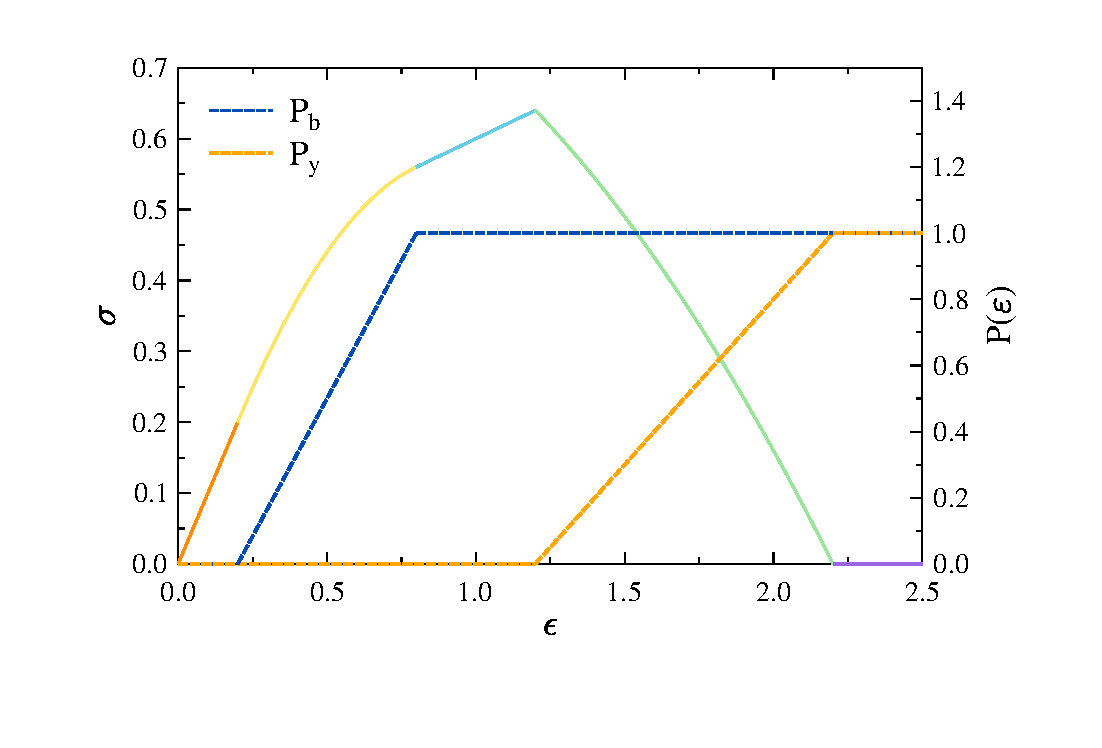
\includegraphics[width=3.4in]{constit4.eps}
    \caption{\label{fig:dust} Inset: mass fraction of non-shattered fragments $S=1-s$ in the final state of the breakup process as a function of strain rate $\dot{\varepsilon}$ for several ring thicknesses $\Delta R/R$. Main panel: Rescaling the curves of the inset by an appropriate power $\nu$ of the ring thickness $\Delta R$, the curves of different $\Delta R$ can be collapsed on a master curve. The black continuous line represents a fit with Eq.\ (\ref{eq:scaling_shatt}). 
    %Note the semi-logarithmic scale on the vertical axis.
    }
\end{figure}

\end{document}
